\chapter{Numerical experiments}

In this chapter we are going to measure the performance of our algorithms by applying them to an example of the weak problem \eqref{weakProb}. For this purpose, the solution of this problem is derived first. Afterwards, we compare the analytical solution with the solution from the FOM-EnOpt and the AML-EnOpt algorithm. Additionally, we examine how the optimization algorithms behave if parameters, such as the step size, are changed or if other neural network training parameters are used.

\section{Example of an analytical problem}

The problem \eqref{weakProb} is solved in \cite{doi:10.1137/070694016} with the adjoint state method \cite{Plessix2006ARO,Becker2007}. For this method, we use the Lagrangian $\mathcal{L}:Q\times X\times X \times V\to\mathbb{R}$ with

\begin{equation}
\label{lagrangian}
\mathcal{L}(q,u,z,\tilde{z})=J(q,u)-(\partial_tu,z)_I-(\nabla u, \nabla z)_I+(f+q, z)_I + (u_0-u(0), \tilde{z})
\end{equation}

We want to find now a stationary point $\bar{q}$ of $j$ such that
\begin{equation}
\label{firstOrderOptimalityCondition}
j'(\bar{q})(\delta_q)=0\quad\forall \delta_q\in Q.
\end{equation}

$j'(\bar{q})(\delta_q)$ is here the directional derivative, which is defined as

\begin{displaymath}
j'(\bar{q})(\delta_q)=\lim_{\tau\downarrow0}\frac{j(q+\tau\delta_q)-j(q)}{\tau}.
\end{displaymath}
If \eqref{firstOrderOptimalityCondition} holds, then $\bar{q}$ satisfies the first order optimality conditions of \eqref{redProb}. In this case, $\bar{q}$ is even optimal due to the linear-quadratic structure of the optimal control problem \cite{doi:10.1137/070694016}.

If we choose $u$ now as $u(q)$, so that it satisfies the weak state equations \eqref{weakProb}, we get

\begin{displaymath}
j(q)=J(q, u(q))=\mathcal{L}(q,u(q),z,\tilde{z}),
\end{displaymath}
since all terms after `$J(q,u)$' in \eqref{lagrangian} are equal to zero.

We get now the directional derivative of $j$ by taking the directional derivative of $\mathcal{L}$ with respect to $q$. We note beforehand that 
\begin{eqnarray*}
-(\partial_tu(q),\delta_z)_I-(\nabla u(q), \nabla \delta_z)_I+(f+q, \delta_z)_I&=&0\quad\forall q\in Q, \delta_z\in X,\\
(u_0-u(q)(0), \delta_{\tilde{z}})&=&0\quad\forall q\in Q, \delta_{\tilde{z}}\in X.
\end{eqnarray*}
By using this, we get the derivative
\begin{equation}
\label{LagrangianDerivative}
\begin{aligned}
j'(q)(\delta_q)=&\mathcal{L}'(q,u(q),z,\tilde{z})(\delta_q)&\\
=&\mathcal{L}'_q(q, u(q), z, \tilde{z})(\delta_q)+\mathcal{L}'_u(q,u(q),z,\tilde{z})(\delta_u).&
\end{aligned}
\end{equation}
%where $\partial_q\mathcal{L}(q, u, z, \tilde{z})(\delta_q)$ is the directional partial derivative of the Lagrangian with respect to $q$ in the direction $\delta_q$.
The first summand in the second line denotes the directional derivative of the Lagrangian with respect to $q$ in direction $\delta_q\in Q$. Analogously, the second summand denotes the directional derivative of the Lagrangian with respect to $u$ in direction $\delta_u\in X$. $\delta_u$ is here uniquely defined such that it satisfies
\begin{equation*}
\begin{aligned}
	(\partial_t\delta_u,\phi)_I+(\nabla \delta_u,\nabla\phi)_I&=(\delta_q,\phi)_I&\forall\phi\in X,\\
	\delta_u(0)&=0&\text{ in }\Omega.
\end{aligned}
\end{equation*}
Then it holds, that for any $\tau\in\mathbb{R}$
\begin{equation*}
\begin{aligned}
	(\partial_t(u(q)+\tau\delta_u),\phi)_I+(\nabla (u(q)+\tau\delta_u),\nabla\phi)_I&=(f+q+\tau\delta_q,\phi)_I&\forall\phi\in X,\\
	(u(q)+\tau\delta_u)(0)&=u_0&\text{ in }\Omega.
\end{aligned}
\end{equation*}
Since $u(q+\tau\delta_q)$ is uniquely defined to satisfy the equations above, it follows that $u(q+\tau\delta_q)=u(q)+\tau\delta_u$.

Therefore we get for every functional $g$ which has a directional derivative in $\delta_u$-direction:
\begin{eqnarray*}
g'_q(u(q))(\delta_q)&=&\lim_{\tau\downarrow0}\frac{g(u(q+\tau\delta_q))-g(u(q))}{\tau}\\
&=&\lim_{\tau\downarrow0}\frac{g(u(q)+\tau\delta_u)-g(u(q))}{\tau}\\
&=&g'_u(u(q))(\delta_u).
\end{eqnarray*}
Because of this, we have the summand $\mathcal{L}'_u(q,u(q),z,\tilde{z})(\delta_u)$ in equation \eqref{LagrangianDerivative}.

We calculate now $\mathcal{L}'_u(q,u,z,\tilde{z})(\delta_u)$. For this we compute $J'_u(q, u)(\delta_u)$ first:
\begin{eqnarray*}
J'_u(q, u)(\delta_u)&=&\lim_{\tau\downarrow0}\frac{1}{2\tau}\int_0^T\int_\Omega(u(t,x)+\tau\delta_u(t, x)-\hat{u}(t,x))^2-(u(t,x)-\hat{u}(t,x))^2\,\mathrm{d}x\,\mathrm{d}t\\
&=&\lim_{\tau\downarrow0}\int_0^T\int_\Omega\delta_u(t, x)(u(t,x)-\hat{u}(t,x))\,\mathrm{d}x\,\mathrm{d}t+\frac{\tau}{2}\int_0^T\int_\Omega(\delta_u(t, x))^2\,\mathrm{d}x\,\mathrm{d}t\\
&=&\int_0^T\int_\Omega\delta_u(t, x)(u(t,x)-\hat{u}(t,x))\,\mathrm{d}x\,\mathrm{d}t=(\delta_u,u-\hat{u})_I
\end{eqnarray*}

We get with similar calculations for the other summands in the Lagrangian:
\begin{equation*}
\mathcal{L}'_u(q,u,z,\tilde{z})(\delta_u)=(\delta_u,u-\hat{u})_I-(\partial_t\delta_u,z)_I-(\nabla\delta_u,\nabla z)_I-(\delta_u(0),\tilde{z}).
\end{equation*}

Since we can choose $z\in X$ and $\tilde{z}\in V$ freely, they are set such that $\mathcal{L}'_u(q,u,z,\tilde{z})(\delta_u)=0$. Integration by parts gives us
\begin{eqnarray*}
&\mathcal{L}'_u(q,u,z,\tilde{z})(\delta_u)&=0\\
\iff&(\delta_u(T),z(T))-(\delta_u(0),z(0))-(\delta_u,\partial_tz)_I+(\nabla\delta_u,\nabla z)_I+(\delta_u(0),\tilde{z})&=(\delta_u,u-\hat{u})_I.
\end{eqnarray*}
This holds if we set $\tilde{z}=z(0)$ and $z$ such that
\begin{equation}
\label{adjoinedStateEquation}
\begin{aligned}
	-(\phi,\partial_tz)_I+(\nabla \phi,\nabla z)_I&=(\phi, u-\hat{u})_I&\forall\phi\in X,\\
	z(T)&=0&\text{ in }\Omega.
\end{aligned}
\end{equation}
We call this the adjoined state equation.

With $z(q)$ defined such as in \eqref{adjoinedStateEquation} and $\tilde{z}(q)=z(q)(0)$, it holds $\mathcal{L}'_u(q,u(q),z(q),\tilde{z}(q))(\delta_u)=0$ and therefore the expression in \eqref{LagrangianDerivative} is equal to
\begin{eqnarray*}
j'(q)(\delta_q)&=&\mathcal{L}'_q(q, u(q), z(q), \tilde{z}(q))(\delta_q)\\
&=&(\alpha q,\delta_q)_I+(z(q),\delta_q)_I\\
&=&(\alpha q+z(q),\delta_q).
\end{eqnarray*}


For the testing of our algorithms, we consider the problem \eqref{weakProb} on $\Omega\times I=(0,1)^2\times(0,0.1)$. The following example is originally described in \cite{doi:10.1137/070694016}.

To define the functions in \eqref{weakProb}, we use the eigenfunction
\begin{displaymath}
w_a(t,x_1,x_2):=\exp(a\pi^2t)\sin(\pi x_1)\sin(\pi x_2) \text{ for } a\in\mathbb{R}.
\end{displaymath}

Now we set

\begin{equation*}
\begin{aligned}
f(t,x_1,x_2)\quad:=\quad&-\pi^4w_a(T,x_1,x_2),&\\
\hat{u}(t,x_1,x_2)\quad:=\quad&\frac{a^2-5}{2+a}\pi^2w_a(t,x_1,x_2)+2\pi^2w_a(T,x_1,x_2),&\\
u_0(x_1,x_2)\quad:=\quad&\frac{-1}{2+a}\pi^2w_a(0,x_1,x_2).&
\end{aligned}
\end{equation*}

If we set the regularization parameter $\alpha$ in the objective functional \eqref{objFun} as $\pi^{-4}$, we get the optimal solution $(\bar{q}, \bar{u}, \bar{z})$, where

\begin{equation}
\label{analyticalSolution}
\begin{aligned}
\bar{q}(t,x_1,x_2)\quad:=\quad&-\pi^4\left(w_a(t,x_1,x_2)-w_a(T,x_1,x_2)\right),&\\
\bar{u}(t,x_1,x_2)\quad:=\quad&\frac{-1}{2+a}\pi^2w_a(t,x_1,x_2),&\\
\bar{z}(t,x_1,x_2)\quad:=\quad&w_a(t,x_1,x_2)-w_a(T,x_1,x_2).&
\end{aligned}
\end{equation}

It holds that $\bar{q}\in Q, \bar{u}\in X, \bar{z}\in X$. We confirm now that $(\bar{q}, \bar{u}, \bar{z})$ is a minimizer by checking if $\bar{q}$ satisfies \eqref{firstOrderOptimalityCondition}, $\bar{u}$ \eqref{weakEq} and $\bar{z}$ \eqref{adjoinedStateEquation}.

Beginning with $\bar{z}$, we have $\bar{z}(T, x_1, x_2)=0$ trivially for all $(x_1,x_2)\in\Omega$. Integration by parts gives for all $\phi\in X$
\begin{displaymath}
(\phi,\partial_tz)_I-(\nabla \phi,\nabla z)_I+(\phi, u-\hat{u})_I=(\phi,\partial_tz+\Delta z+u-\hat{u})_I.
\end{displaymath}
Now we compute
\begin{eqnarray*}
\partial_t\bar{z}(t,x_1,x_2)&=&\partial_tw_a(t,x_1,x_2)=a\pi^2w_a(t,x_1,x_2)\\
\Delta \bar{z}(t,x_1,x_2)&=&2\pi^2(w_a(T,x_1,x_2)-w_a(t,x_1,x_2))\\
\bar{u}(t,x_1,x_2)-\hat{u}(t,x_1,x_2)&=&\pi^2((2-a)w_a(t,x_1,x_2)-2w_a(T,x_1,x_2)).
\end{eqnarray*}
From $\partial_t\bar{z}(t,x_1,x_2)+\Delta \bar{z}(t,x_1,x_2)+\bar{u}(t,x_1,x_2)-\hat{u}(t,x_1,x_2)=0$ for all $(x_1,x_2)\in\Omega, t\in I$ follows that $\bar{z}$ satisfies the adjoined state equation \eqref{adjoinedStateEquation}.

By doing the same for $\bar{u}$, we see that it meets the initial condition $\bar{u}(0,x_1,x_2)=u_0(x_1,x_2)$ for all $(x_1,x_2)\in\Omega$ of \eqref{weakEq}. Again, integration by parts gives us for all $\phi\in X$
\begin{displaymath}
(\partial_t\bar{u},\phi)_I+(\nabla \bar{u},\nabla\phi)_I-(f+\bar{q},\phi)_I=(\partial_t\bar{u}-\Delta\bar{u}-f-\bar{q},\phi)_I.
\end{displaymath}
It holds
\begin{eqnarray*}
\partial_t\bar{u}(t,x_1,x_2)&=&\frac{-a}{2+a}\pi^4w_a(t,x_1,x_2)\\
\Delta \bar{u}(t,x_1,x_2)&=&\frac{2}{2+a}\pi^4w_a(t,x_1,x_2)\\
\partial_t\bar{u}(t,x_1,x_2)-\Delta \bar{u}(t,x_1,x_2)&=&-\pi^4w_a(t,x_1,x_2)\\
&=&f(t,x_1,x_2)+\bar{q}(t,x_1,x_2).
\end{eqnarray*}
Therefore $\partial_t\bar{u}(t,x_1,x_2)-\Delta\bar{u}(t,x_1,x_2)-f(t,x_1,x_2)-\bar{q}(t,x_1,x_2)=0$ for all $(x_1,x_2)\in\Omega, t\in I$, so $\bar{u}$ fulfills the conditions in the weak state equation \eqref{weakEq}.

With $\alpha=\pi^{-4}$ we get $\alpha\bar{q}(t,x_1,x_2)+\bar{z}(t,x_1,x_2)=0$ for all $(x_1,x_2)\in\Omega, t\in I$, which means that $\bar{q}$ satisfies the optimality condition \eqref{firstOrderOptimalityCondition}. Now we conclude that $(\bar{q}, \bar{u}, \bar{z})$ is the optimal solution.\\

Since the solutions $q\in Q_d$ of our algorithms have the form that is described in \eqref{discrContrVar}, we need to define a control-shape functional before we search for an optimizer. $\bar{q}$ can be written as
\begin{displaymath}
\bar{q}(t,x_1,x_2)=-\pi^4(\exp(a\pi^2t)-\exp(a\pi^2T))\sin(\pi x_1)\sin(\pi x_2).
\end{displaymath}
Now we have $\bar{q}$ as a product of the term $-\pi^4(\exp(a\pi^2t)-\exp(a\pi^2T))$, that is only dependent on $t$, and the shape functional $\sin(\pi x_1)\sin(\pi x_2)$, which depends only on $x$ and is an element of $H$. Additional shape functionals for the control functional are not used so that we can compare the output of our optimization algorithms with the analytical solution $\bar{q}$. We expect that the elements $q^i_1$ of the control vectors $\mathbf{q}$ that we get as outputs are close to
\begin{equation}
\label{controlVectorElements}
\bar{q}^i_1=-\pi^4(\exp(a\pi^2t_i)-\exp(a\pi^2T))\text{ for }i=0,\dotsc,M.
\end{equation}
For our tests, we choose $a$ to be $-\sqrt{5}$, so that $f$ and $\hat{u}$ do not depend on time.

\section{Numerical results}

Now we test the FOM- and AML-EnOpt algorithms on the example from the last section. We discretize the space $\Omega=(0,1)^2$ as described in subsection \ref{SubsectionDiscretizationInSpace} with $50$ grid intervals. The time interval $I=(0,T)$ with $T=0.1$ that we observe is divided into $10$ smaller intervals which are all of the same size. This is described in subsection \ref{SubsectionDiscretizationInTime} with $M=10$. Since we have only one shape functional, the control vectors $\mathbf{q}$ that we search for have $N_\mathbf{q}=11$ elements.

The initial control vector $\mathbf{q}_0$ is a vector with constant entries of the value $-40$. This value lies approximately between the minimum element in \eqref{controlVectorElements} which is $\bar{q}^0_1\approx-87$ and the maximum $\bar{q}^M_1=0$. The values of the constant initial control vector, along with other parameters for the algorithms that are presented in the chapters \ref{ChapterEnsembleBasedOptimizationAlgorithm} and \ref{ChapterAdaptiveMLEnOptAlgorithm}, are specified in the table \ref{FOMAMLEnOptParameters}. The notation in the table corresponds to the notation in these algorithms.

The neural network that is used for the surrogate functional consists of two hidden layers where each hidden layer has $25$ neurons. Our activation function is the $\tanh$ function as mentioned in section \ref{sectionDeepNeuralNetworks}. Early stopping is applied for the training of the DNN with a maximum of $1000$ training epochs. The variable $\mathrm{earlyStop}$ in algorithm \ref{trainDNN} is set to $20$. We use the L-BFGS optimizer with strong Wolfe line-search for the minimization of the MSE loss on the validation set. The validation set consists of $20\%$ of the sample set, so the other $80\%$ of the sample set are used for the training set. The number of training restarts is very small because a higher number would extend the training time of the DNN by so much that it makes the algorthm terminate slower. We restart the training two times, so we train three DNNs in total to construct the surrogate functional.

Before the results are presented, we want to remember that the FOM-EnOpt and the Adaptive-ML-EnOpt procedures minimize the objective functional $j$ by maximizing the negative functional $-j$. The results that we show are converted back to the outputs that the objective functional $j$ would give, although the true values during these algorithms are negative. As an example, the graphs in figure \ref{FOMAMLEnOptFuncValComp} would be mirrored on the y-axis if they had shown the values during the respective procedure.

For consistency, we will refer to $\mathbf{q}_k$ as the iterate at the beginning of the outer iteration $k$ and $\mathbf{q}^\mathrm{next}_k$ as the iterate at the end of the outer iteration $k$. This is based on the notation of the AML-EnOpt algorithm \ref{AML-EnOpt}. If we talk about the FOM-EnOpt algorithm, we refer to $\mathbf{q}_k$ as the iterate before the call of the optimization step procedure in line \ref{EnOptAlgOptStepCall1}, respectively line \ref{EnOptAlgOptStepCall2}, in the $k$-th outer iteration of the algorithm \ref{EnOptAlg} and thus we denote $\mathbf{q}^\mathrm{next}_k$ as the iterate after this call in iteration $k$.

\begin{table}[h]
%\footnotesize
\caption{\label{FOMAMLEnOptParameters}Parameters used in the FOM-EnOpt and AML-EnOpt algorithms}
\centering
\begin{tabular}{ll}
\hline
Parameter & Value\\
\hline
Elements of the initial constant control vector $\mathbf{q}_0$ & -40\\
Initial step size $\beta_1$ & $1$\\
Initial covariance matrix adaption step size $\beta_2$ & $0.1$\\
Initial trust region step size $\delta_\mathrm{init}$ & $100$\\
Step size contraction $r$ & $0.5$\\
Maximum step size trials $\nu^*$ & $10$\\
Maximum (outer/ inner) iterations $k^*, k^*_o, k^*_i$ & $1000$\\
Maximum trust region iterations $k^*_\mathrm{TR}$ & $5$\\
Initial control-type variance $\sigma^2_1$ & $0.1$\\
Constant correlation factor $\rho$ & $0.9$\\
Perturbation size $N$ & $100$\\
FOM-EnOpt $\varepsilon$ & $10^{-8}$\\
Tolerances Adaptive-ML-EnOpt inner iteration $\varepsilon_i$ & $10^{-12}$\\
Adaptive-ML-EnOpt outer iteration $\varepsilon_o$ & $10^{-8}$\\
%& $$\\
\hline
\end{tabular}
\end{table}

Figure \ref{FOMAMLEnOptFuncValComp} shows the development of the FOM objective functional value $\Call{j}{\mathbf{q}^\mathrm{next}_k}$ after each outer iteration during the FOM- and AML-EnOpt procedures, as well as the respective functional value $\Call{j$^k_\mathrm{ML}$}{\mathbf{q}^\mathrm{next}_k}$ of the surrogate functional $\textproc{j$_\mathrm{ML}^k$}$ that is used in line \ref{innerIterationCallAlgo} of the AML-EnOpt algorithm \ref{AML-EnOpt} to compute the iterate $\mathbf{q}^\mathrm{next}_k$.% We want to emphasize here that we specifically mean the iterate $\mathbf{q}_k$ at the end of each outer iteration. So in plots of the AML-EnOpt algorithm, we reference the $\mathbf{q}_k$ that is set in line \ref{AMLSetqk}.

We can see here that the functional values of the FOM-EnOpt and the Adaptive-ML-EnOpt algorithms converge towards a minimum. The output of the FOM-EnOpt algorithm gives an output whose objective functional value is approximately $4.22982802$ after $125$ iterations. The FOM objective functional value of the output from the AML-EnOpt procedure is approximately $4.22981359$ which is reached after only $25$ outer iterations. So the Adaptive-EnOpt algorithm gives here not only an output that has a smaller objective functional value, but also requires far fewer outer iterations than the FOM-EnOpt algorithm to terminate.\\

To compare the functional values of the objective functional and the surrogate functionals of the Adaptive-ML-EnOpt procedure, we examine figure \ref{AMLEnOptFuncValComp}. The plot at the top shows the same graphs as in figure \ref{FOMAMLEnOptFuncValComp}, except that the objective functional values of the FOM-EnOpt algorithm are not included. The plot at the bottom shows only the last five outer iterations of the plot from above. We can see here that there is quite a big difference between the objective functional values and the surrogate functional values in the first outer iterations. The difference after the first iteration is approximately $0.02$. However, this difference gets smaller during the runtime of the procedure and is in the order of $10^{-7}$ for the last iterations.

One reason for this phenomenon is the difference between $\mathbf{q}_k$ and $\mathbf{q}^\mathrm{next}_k$ at different outer iterations. In the first iterations, we are relatively far away from an optimum and therefore the iterates change considerably. The surrogate functional is trained by a training and a validation set which are sampled around the iterate $\mathbf{q}_k$, so  if the difference between $\mathbf{q}^\mathrm{next}_k$ and $\mathbf{q}_k$ is large, the same tends to hold for the difference between $\mathbf{q}^\mathrm{next}_k$ and the samples, so the surrogate functional is less precise at $\mathbf{q}^\mathrm{next}_k$. As the algorithm progresses, the iterate converges towards an optimum and the differences between successive iterates are smaller, resulting in more accurate surrogate functional values.

This can be seen in figure \ref{L2Dist}. In the first iteration, the step from $\mathbf{q}_k$ to $\mathbf{q}^\mathrm{next}_k$ is much larger than the step from $\mathbf{q}_k$ to $\tilde{\mathbf{q}}_k$. The same holds with regard to the difference between $\mathbf{q}_k$ and the samples in $T_k$. Therefore the DNN is inaccurate at $\mathbf{q}^\mathrm{next}_k$. If this were the FOM-EnOpt algorithm, then $\tilde{\mathbf{q}}_k$ would be the next iterate, so we can see here a reason why the AML-EnOpt algorithm requires far fewer iterations than the FOM-EnOpt procedure which is that the machine learning-based algorithm takes larger steps at the beginning.

Although the step from $\mathbf{q}_k$ to $\mathbf{q}^\mathrm{next}_k$ is still larger than the step from $\mathbf{q}_k$ to $\tilde{\mathbf{q}}_k$ at the last iteration, the step sizes differ not by a lot compared to the first iteration. $\mathbf{q}^\mathrm{next}_k$ is even closer to $\mathbf{q}_k$ than all the samples are since the value of $\mathbf{q}^\mathrm{next}_k$ at the bottom plot in figure \ref{L2Dist} is smaller than the value of $T_k$ min which is the sample in $T_k$ with the minimum $L^2$-distance to $\mathbf{q}_k$.\\

Figure \ref{FOMAMLEnOptSolutionComp} shows the solutions that we get from the FOM-EnOpt and the Adaptive-ML-EnOpt algorithms, as well as the analytical solution and the initialization of the iterates at the top. At the bottom, the difference between the FOM-EnOpt, respectively AML-EnOpt, solution and the analytical solution is depicted. The plot at the bottom shows us that the two solutions strategies yield similar results. At most points, the solutions of both algorithms are relatively close to the analytical solution. However, the control values for the second, last and especially first time step are far from the analytically optimal values.

A reason for this might be inaccuracies of the state variable discretizations. The objective functional is calculated according to subsection \ref{subsectionCalculationOfTheObjectiveFunctionValue} as

\begin{equation}
\label{discretizedObjectiveFunctionalRep}
\begin{aligned}
\frac{T}{6M}\sum_{m=1}^M&\left(U_{m-1}-\hat{U}_{m-1}\right)M_n\left(U_{m-1}-\hat{U}_{m-1}\right)\\
&+ \left(U_{m-1}-\hat{U}_{m-1}\right)M_n\left(U_{m}-\hat{U}_{m}\right)\\
&+ \left(U_{m}-\hat{U}_{m}\right)M_n\left(U_{m}-\hat{U}_{m}\right)\\
+ \frac{\alpha T}{6M}\sum_{m=1}^M&Q_{m-1}M_nQ_{m-1} + Q_{m-1}M_nQ_{m} + Q_{m}M_nQ_{m},
\end{aligned}
\end{equation}
where the notation corresponds to the notation of subsection \ref{subsectionCalculationOfTheObjectiveFunctionValue}.

We compute the state variables $U_m$ with the Crank-Nicolson scheme \eqref{crank_nicolson}:
\begin{equation*}
\left(\tilde{M}_n^T + \frac{T}{2M} \tilde{L}_n^T\right) U_m = \tilde{M}_n^TU_{m-1} - \frac{T}{2M} \tilde{L}_n^T U_{m-1} + \frac{T}{2M} F_{m-1} + \frac{T}{2M} F_m,
\end{equation*}
for $m=1,\dotsc,M$. The control $q^m_1$ influences only the vector $F_m$ directly for $m=0,\dotsc,M$. Hence, for $m=1,\dotsc,M-1$, each control $q^m_1$ is used for the definitions of the states $U_m$ and $U_{m+1}$. Only $q^0_1$ and $q^M_1$ set just one state which is $U_1$, respectively $U_M$, while they are still weighted with the same value of $\frac{T}{2M}$ as every other control. Therefore changes of $q^0_1$ and $q^M_1$ tend to effect the first part of \eqref{discretizedObjectiveFunctionalRep} less than the other control variables. Hence, the control variables may reduce the regularization term in \eqref{discretizedObjectiveFunctionalRep} instead by going closer to zero. This can be seen for $q^0_1$. The first control of the analytical solution is approximately $\bar{q}^0_1\approx-87$ which is far from zero. Therefore, with the discretization, it might be beneficial to reduce the regularization term by increasing $q^0_1$. Since the difference $q^0_1$ and $\bar{q}^0_1$ is so large, it is not surprising that $q^1_1$ is also not a good approximation of $\bar{q}^1_1$. In contrast to $q^0_1$, $q^M_1$ is further away from zero than its respective control of the analytical solution. However, due to the quadratic nature of the regularization term, this has not such a strong effect on the objective functional. To reduce these inaccuracies, we could increase the number of time steps. This is examined further below.\\

\begin{figure}
\centering
%\textbf{Your title}\par\medskip
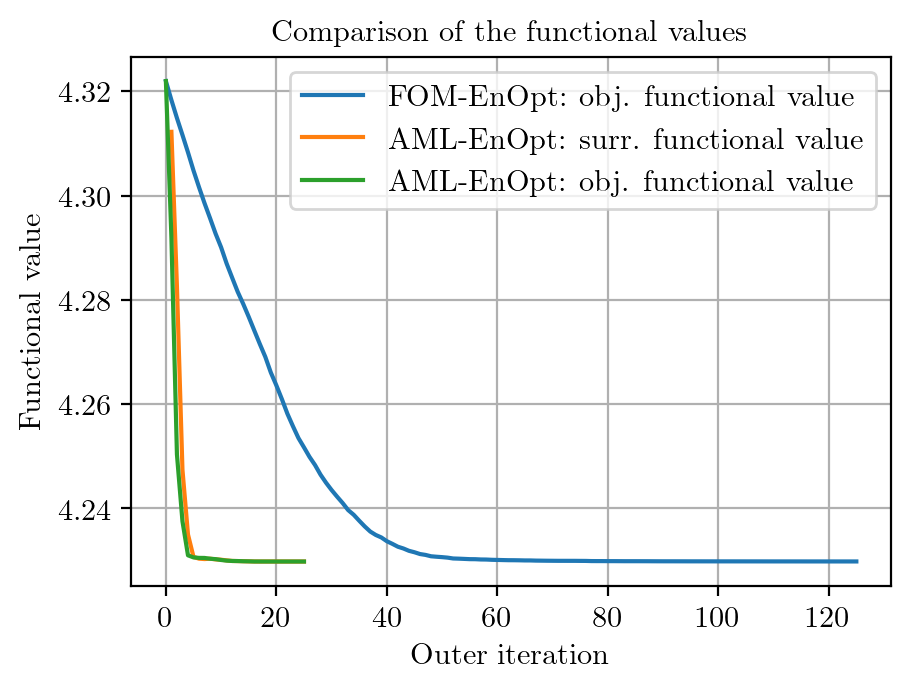
\includegraphics{Plots/functionalValueComp.png}
\caption{\label{FOMAMLEnOptFuncValComp}Comparison of the FOM objective functional values obtained during the outer iterations of the FOM-EnOpt and AML-EnOpt algorithms, as well as the surrogate functional values obtained during the outer iterations of the AML-EnOpt algorithm}
\end{figure}

\begin{figure}
\centering
%\textbf{Your title}\par\medskip
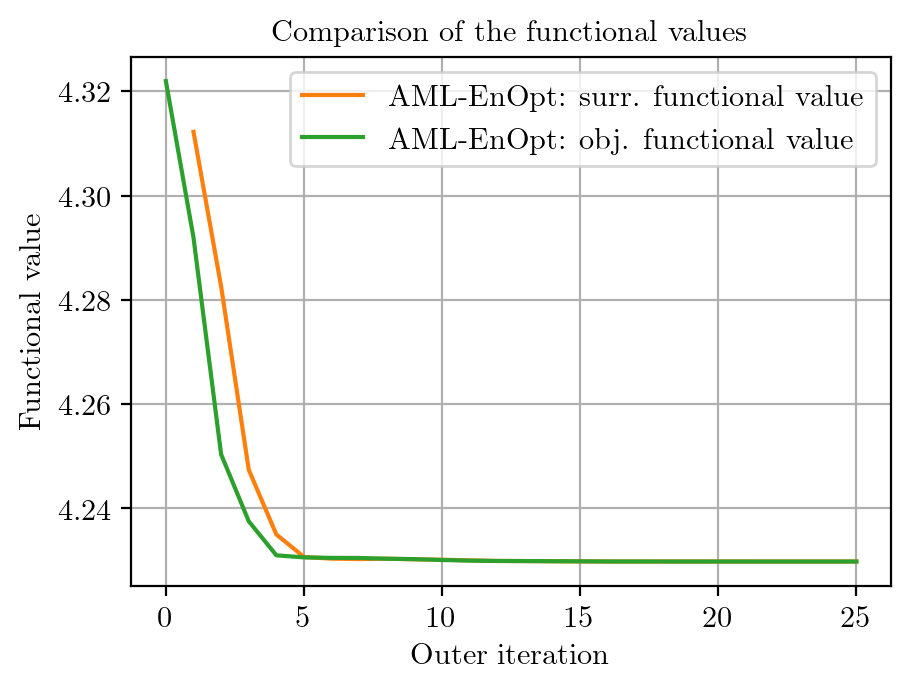
\includegraphics{Plots/reducedFunctionalValueComp.png}
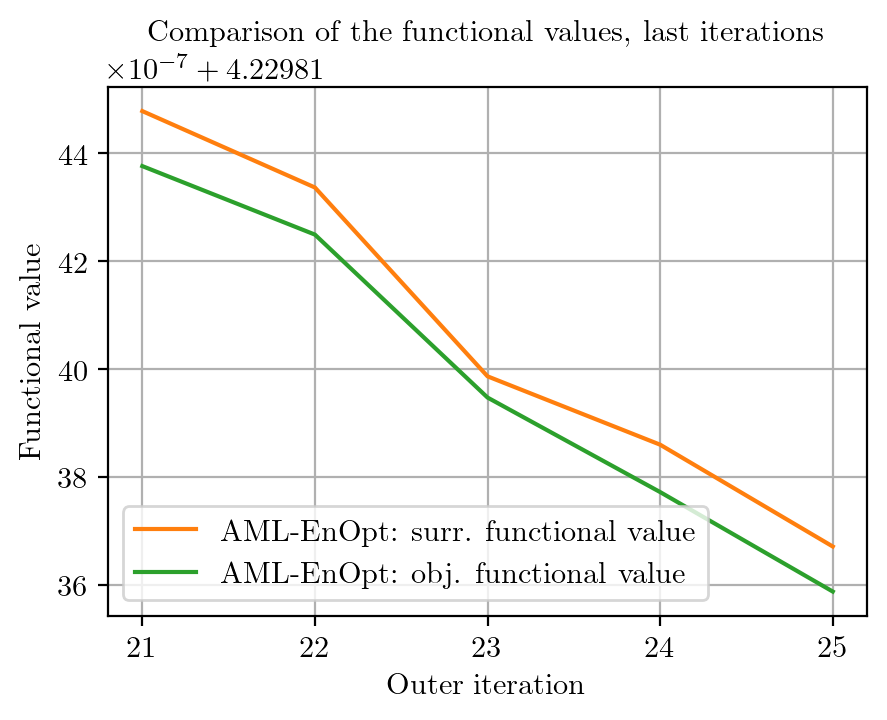
\includegraphics{Plots/reducedFunctionalValueCompLastIter.png}
\caption{\label{AMLEnOptFuncValComp}Comparison of the FOM objective functional values obtained during the outer iterations of the AML-EnOpt algorithm, as well as the respective surrogate functional values}
\end{figure}

\begin{figure}
\centering
%\textbf{Your title}\par\medskip
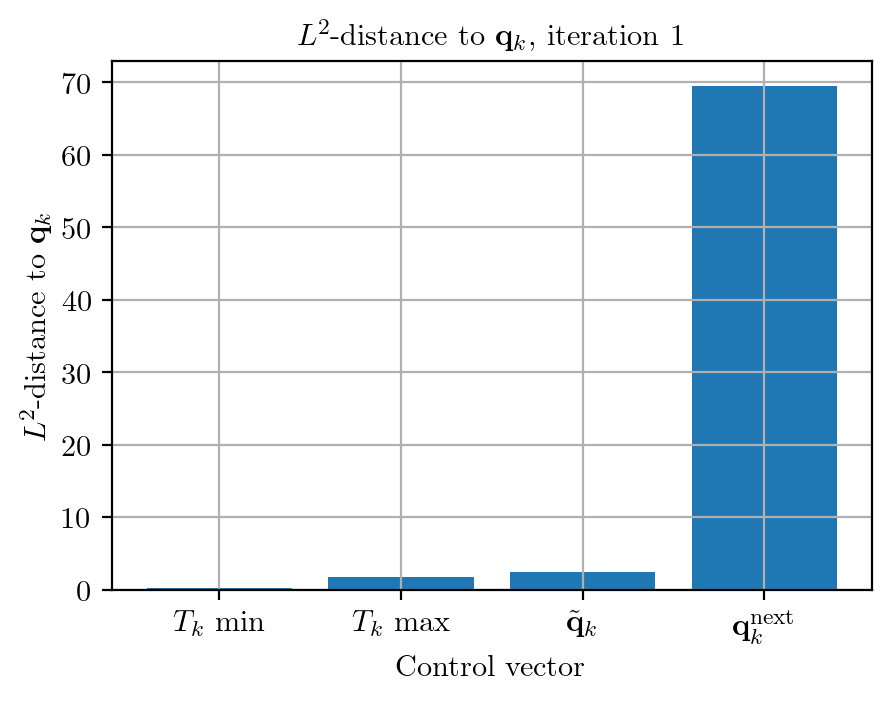
\includegraphics{Plots/firstL2Dist.png}
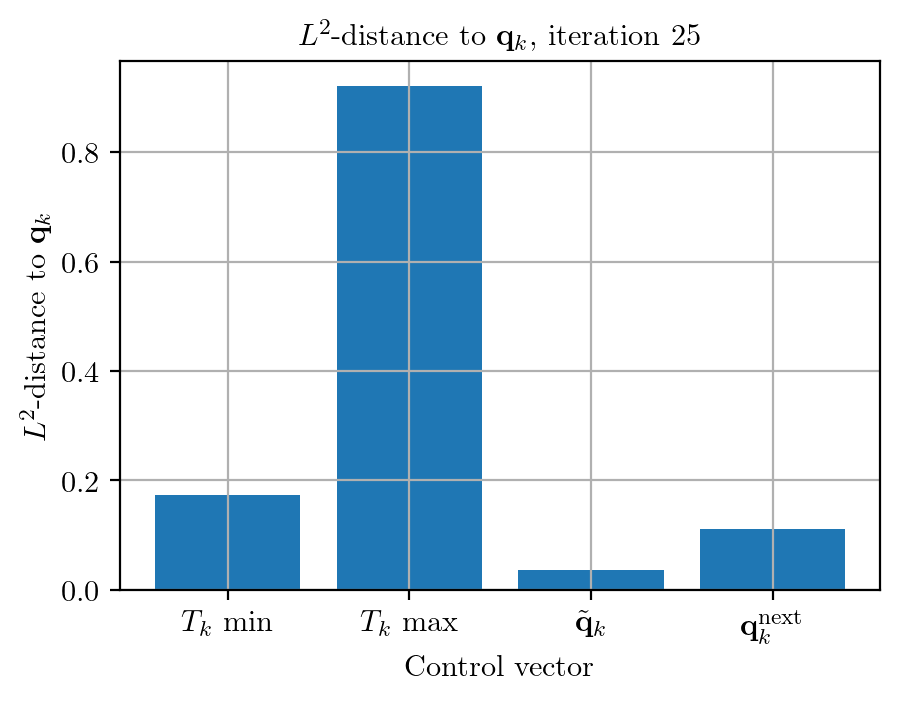
\includegraphics{Plots/lastL2Dist.png}
\caption{\label{L2Dist}$L^2$-distance between $\mathbf{q}_k$ and $T_k$ min, $T_k$ max, $\tilde{\mathbf{q}}_k$ and $\mathbf{q}^\mathrm{next}_k$ at the first (top) and last (bottom) outer iteration. $\mathbf{q}_k$ is here the iterate at the start of the respective iteration and $\mathbf{q}^\mathrm{next}_k$ the iterate at the end of the iteration. $T_k$ min is the sample in $T_k$ with the minimum $L^2$-distance to $\mathbf{q}_k$ and $T_k$ max the sample with the maximum $L^2$-distance to $\mathbf{q}_k$.}
\end{figure}

\begin{table}[h]
\caption{\label{resultComparison}Comparison of the results from the FOM-EnOpt and AML-EnOpt algorithms}
%\footnotesize
\centering
\begin{tabular}{|l|l|l|l|}
\hline
Method & Iteration & FOM objective function value  & Surrogate function value \\%& FOM eval. & Surrogate eval. & Training time (min) & $T_\mathrm{total}$ (min) & Speedup\\
\hline
\hline
$\mathrm{FOM-EnOpt}$ & $1$ & $4.229826194856661$ & - \\%& $2839$ & - & - & $54.86$ & - \\
\cline{2-4}
 & $2$ & $4.229829269880319$ & - \\%& $2839$ & - & - & $54.86$ & - \\
\cline{2-4}
 & $3$ & $4.2298361817288885$ & - \\%& $2839$ & - & - & $54.86$ & - \\
 \hline
$\mathrm{AML-EnOpt}$ & $1$ & $4.229813297937858$ & $4.229813485631982$ \\%& $407$ & $12315$ & $2.03$ & $8.87$ & $6.18$ \\
\cline{2-4}
 & $2$ & $4.229813596812994$ & $4.229813708587202$ \\%& $2839$ & - & - & $54.86$ & - \\
\cline{2-4}
 & $3$ & $4.229813126525124$ & $4.22981328826163$ \\%& $2839$ & - & - & $54.86$ & - \\
\hline
\multicolumn{4}{l}{}\\
\hline
Method & Iteration & Outer iterations  & Inner iterations \\%& FOM eval. & Surrogate eval. & Training time (min) & $T_\mathrm{total}$ (min) & Speedup\\
\hline
\hline
$\mathrm{FOM-EnOpt}$ & $1$ & $119$ & - \\%& $2839$ & - & - & $54.86$ & - \\
\cline{2-4}
 & $2$ & $114$ & - \\%& $2839$ & - & - & $54.86$ & - \\
\cline{2-4}
 & $3$ & $124$ & - \\%& $2839$ & - & - & $54.86$ & - \\
 \hline
$\mathrm{AML-EnOpt}$ & $1$ & $27$ & $924$ \\%& $407$ & $12315$ & $2.03$ & $8.87$ & $6.18$ \\
\cline{2-4}
 & $2$ & $27$ & $877$ \\%& $2839$ & - & - & $54.86$ & - \\
\cline{2-4}
 & $3$ & $24$ & $895$ \\%& $2839$ & - & - & $54.86$ & - \\
\hline
\multicolumn{4}{l}{}\\
\hline
Method & Iteration & FOM evaluations  & Surrogate evaluations \\%& FOM eval. & Surrogate eval. & Training time (min) & $T_\mathrm{total}$ (min) & Speedup\\
\hline
\hline
$\mathrm{FOM-EnOpt}$ & $1$ & $12107$ & - \\%& $2839$ & - & - & $54.86$ & - \\
\cline{2-4}
 & $2$ & $11629$ & - \\%& $2839$ & - & - & $54.86$ & - \\
\cline{2-4}
 & $3$ & $12643$ & - \\%& $2839$ & - & - & $54.86$ & - \\
 \hline
$\mathrm{AML-EnOpt}$ & $1$ & $2912$ & $95047$ \\%& $407$ & $12315$ & $2.03$ & $8.87$ & $6.18$ \\
\cline{2-4}
 & $2$ & $2905$ & $90241$ \\%& $2839$ & - & - & $54.86$ & - \\
\cline{2-4}
 & $3$ & $2589$ & $91967$ \\%& $2839$ & - & - & $54.86$ & - \\
\hline
\multicolumn{4}{l}{}\\
\hline
Method & Iteration & Total run time (min) & Training time (min)\\%& FOM eval. & Surrogate eval. & Training time (min) & $T_\mathrm{total}$ (min) & Speedup\\
\hline
\hline
$\mathrm{FOM-EnOpt}$ & $1$ & $37.67$ & -  \\%& $2839$ & - & - & $54.86$ & - \\
\cline{2-4}
 & $2$ & $36.07$ & - \\%& $2839$ & - & - & $54.86$ & - \\
\cline{2-4}
 & $3$ & $39.22$ & - \\%& $2839$ & - & - & $54.86$ & - \\
 \hline
$\mathrm{AML-EnOpt}$ & $1$ & $24.05$ & $14.24$ \\%& $407$ & $12315$ & $2.03$ & $8.87$ & $6.18$ \\
\cline{2-4}
 & $2$ & $23.87$ & $14.17$ \\%& $2839$ & - & - & $54.86$ & - \\
\cline{2-4}
 & $3$ & $22.14$ & $13.39$ \\%& $2839$ & - & - & $54.86$ & - \\
\hline
\end{tabular}
\end{table}



%\begin{figure}
%\centering
%%\textbf{Your title}\par\medskip
%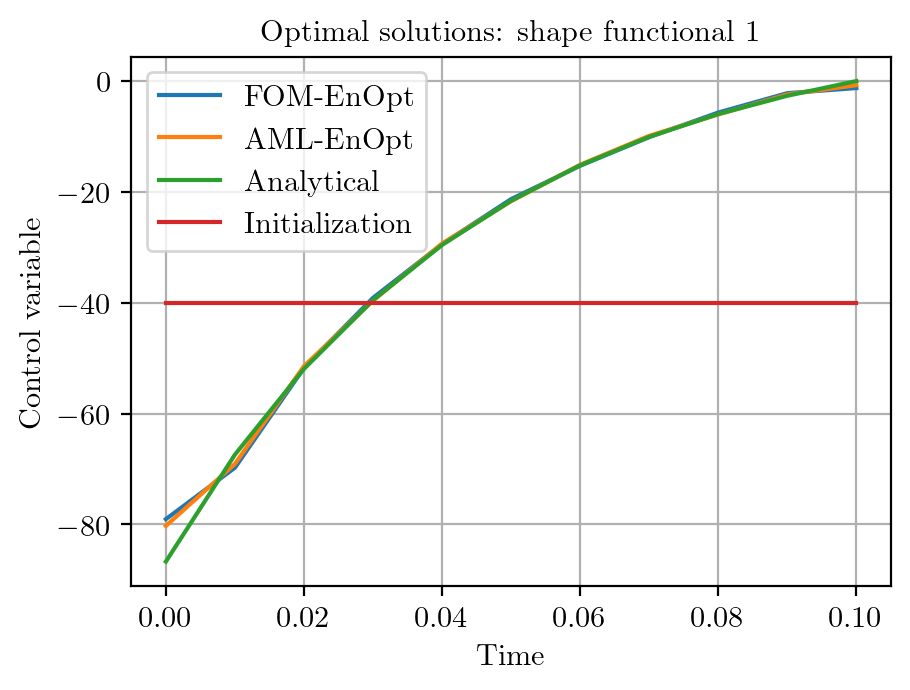
\includegraphics[height=5.7cm]{Plots/solutions.png}
%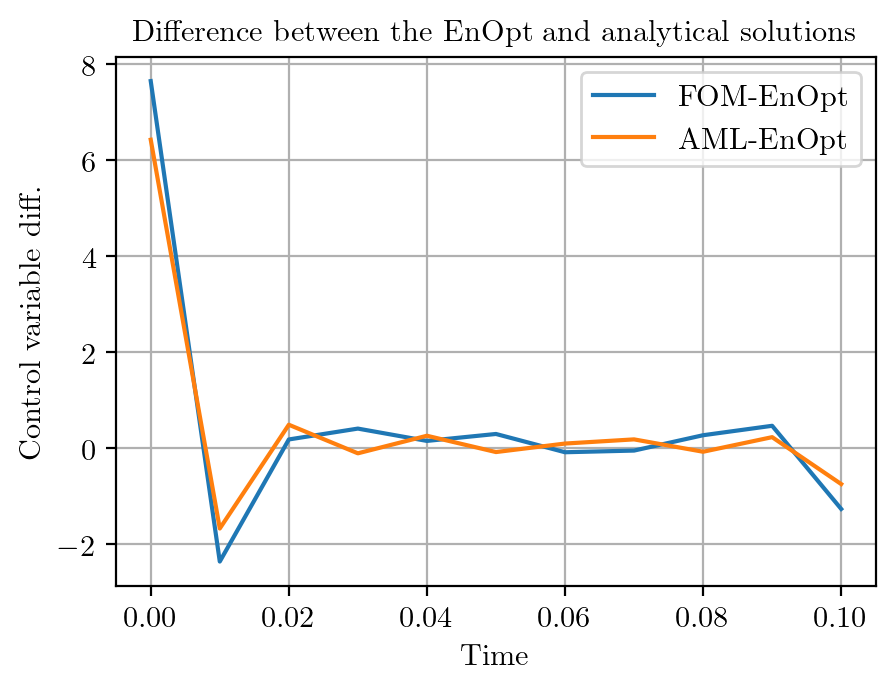
\includegraphics[height=5.7cm]{Plots/solutionsDiffer.png}
%\caption{Comparison of the optimal solutions obtained from the FOM-EnOpt and the AML-EnOpt algorithms}
%\end{figure}

\begin{figure}
\centering
%\textbf{Your title}\par\medskip
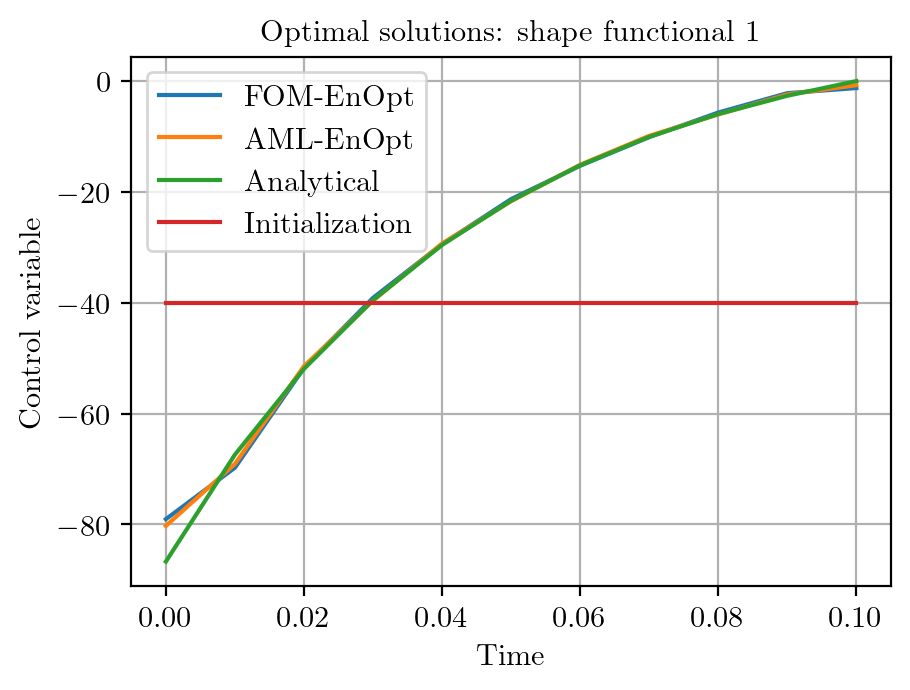
\includegraphics{Plots/solutions.png}
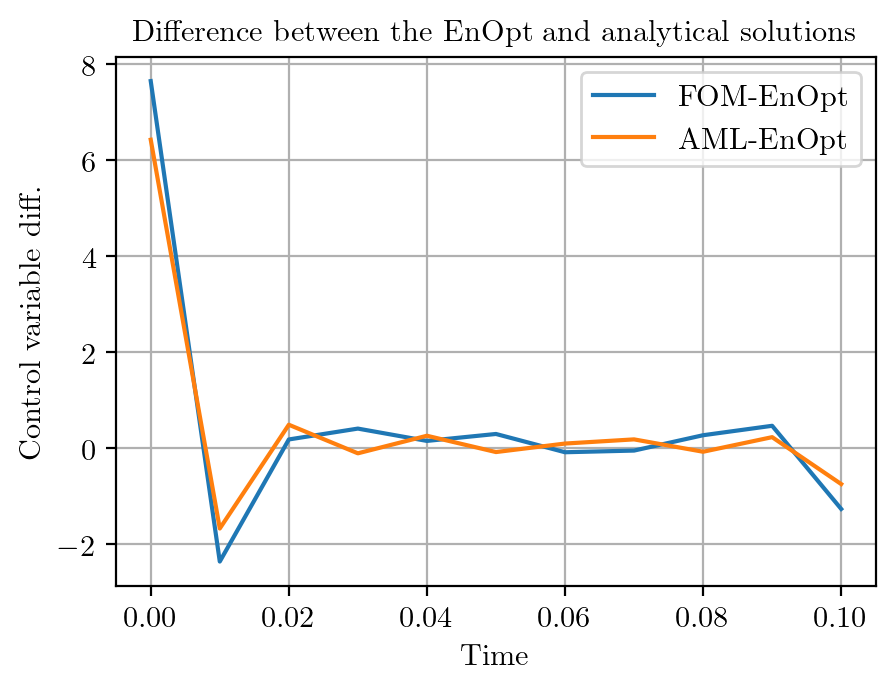
\includegraphics{Plots/solutionsDiffer.png}
\caption{\label{FOMAMLEnOptSolutionComp}Comparison of the optimal solutions obtained from the FOM-EnOpt and the AML-EnOpt algorithms}
\end{figure}

To investigate the effects of different neural network structures, we test now the AML-EnOpt algorithm with different quantities of neurons in the hidden layer. The number of hidden layers is fixed to two. The progression of the FOM objective functional values for different DNN structures is shown in Figure \ref{DNNStructComparison}. To distinguish the different results, the bottom plot shows the objective functional values of the last outer iterations. Since the procedure with $1000$ neurons in the hidden layer has here many more outer iterations than the rest, we do not show this plot to make the differences between the other results clearer. The number of outer iterations, as well as the minimum, maximum, and average training and validation losses are shown in table \ref{DNNLossComparison}. The values in the table \ref{DNNStructFOMComparison}, multiplied with $10^{-5}$ and added to $4.2298$, are the FOM objective functional values that the outputs of the respective procedures yields.\\

The initial shape functional control variance $\sigma^2_1$ and the constant correlation factor $\rho$ have a strong effect on the runtime and output of the FOM-EnOpt and AML-EnOpt algorithms. If the variance is too large, the FOM-EnOpt procedure tends to give a worse optimal solution. If the variance is too small, this algorithm needs more optimization steps than necessary to terminate.

We choose the correlation factor to be close to one so that we get a smoother output. However, if this value is too large, the result is similar to a large $\sigma^2_1$ which we want to avoid. For example, if we set $\rho=0.9$, we get from \eqref{defineInitialCovariance} that the variance of $q^i_1$ is approximately $5.3\cdot\sigma^2_1$ for $i=0,\dotsc,M$. If $\rho$ is equal to $0.99$, the variance is with a value of approximately $50.3\cdot\sigma^2_1$ almost ten times as high.

A poor choice of these values may have even more serious consequences for the FOM-EnOpt algorithm. If we set the variance too small, the neural network-based surrogate functional is not approximating the FOM objective functional sufficiently well in a large enough area and the AML-EnOpt algorithm fails. However, we still want to set the variance so small that the surrogate is a good approximation of the objective functional in a small area around the iterate when we are close to the optimal solution.

We conclude that $\sigma^2_1$ and $\rho$ should be chosen carefully and dependent on each other. If we increase $\rho$ to get smoother iterates, we might have to decrease $\sigma^2_1$ so that the area which contains our samples is not too large. Hence, it might require some testing to find values that suit the available optimization problem.\\

Unlike the Adaptive-ML-EnOpt algorithm in \cite{Keil2022-dj}, we need to employ a trust region method. If we proceed without it, we get the results of figure \ref{noTRResults}. The method seems to work up to the eighth iteration, but the machine learning-based surrogate suggests in the ninth outer iteration that there is an optimum near a point that is far from the actual optimum. This point is shown in the bottom plot of figure \ref{noTRResults}. Some entries of the resulting control vector exceed even the value of $600$, although they should be below zero.

\begin{figure}
\centering
%\textbf{Your title}\par\medskip
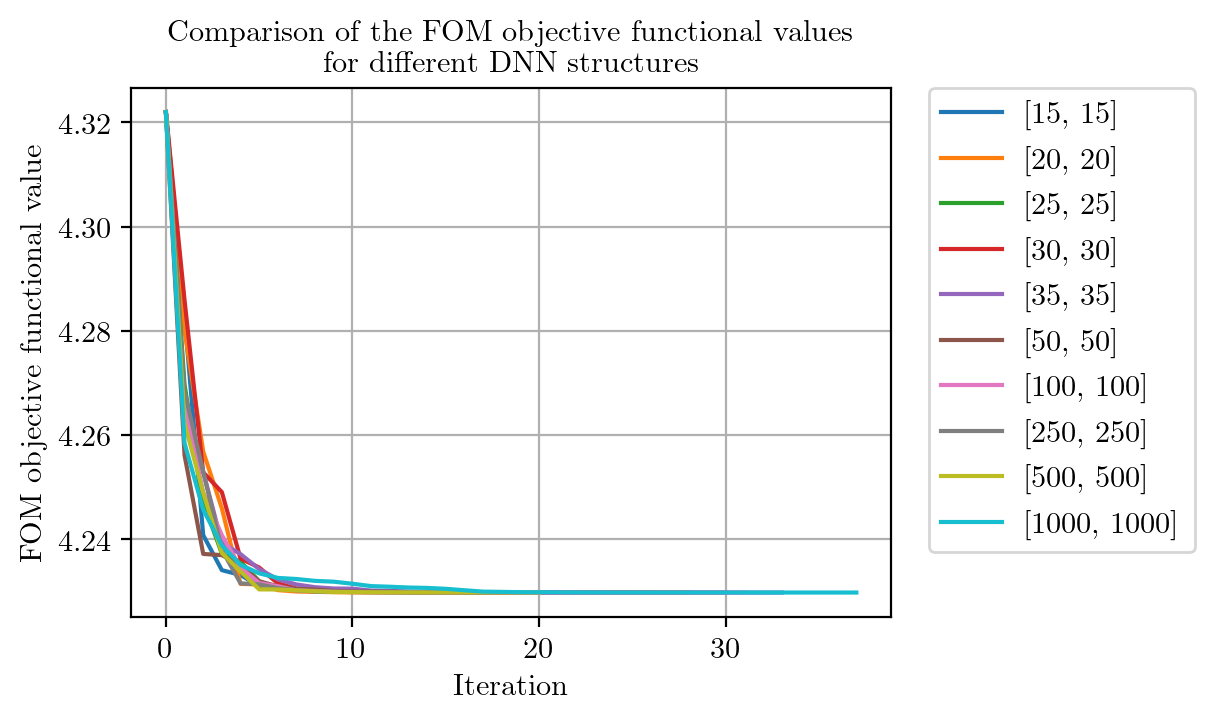
\includegraphics{Plots/DNNStruct.png}
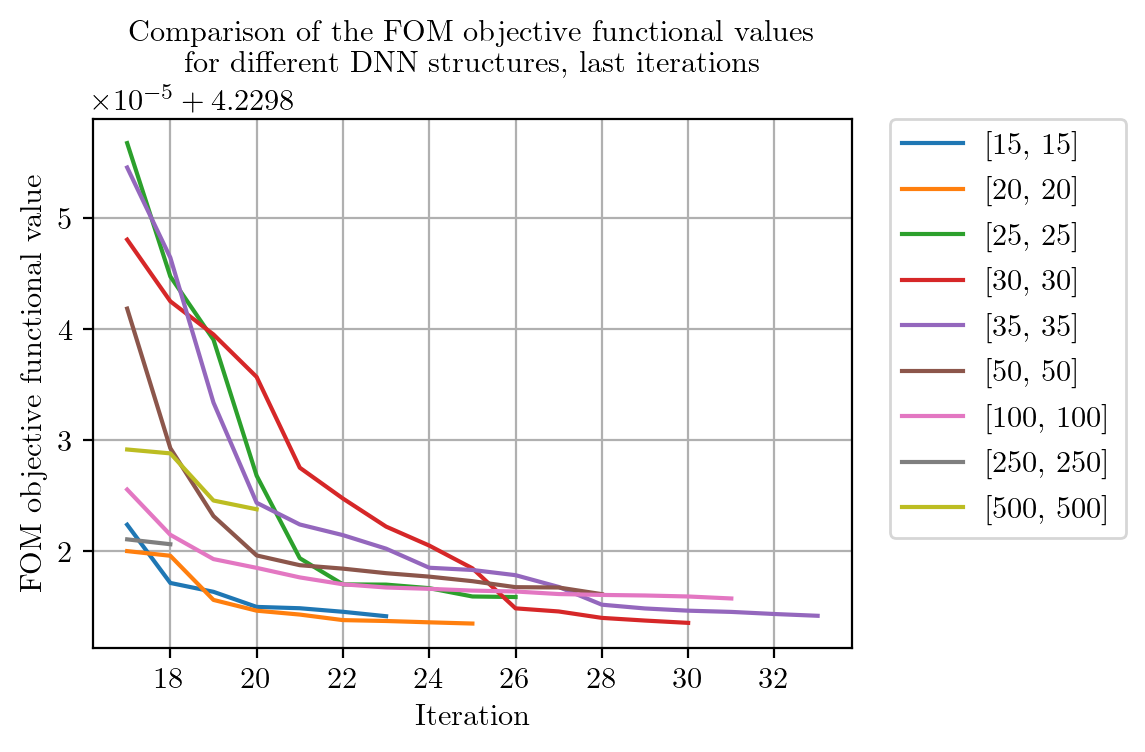
\includegraphics{Plots/DNNStructLastIter.png}
\caption{\label{DNNStructComparison}Comparison of the FOM objective functional values from the AML-EnOpt algorithm for different numbers of neurons in the hidden layers. The plot at the bottom shows the functional values of the last outer iterations without the result with $1000$ neurons in the hidden layers.}
\end{figure}


\begin{table}[h]
\caption{\label{DNNLossComparison}Minimum, maximum, and average MSE loss on the training and validation set during the AML-EnOpt procedure with different numbers of neurons in the hidden layers of the neural network. The number of hidden layers is fixed to two.}
%\footnotesize
\centering
\begin{tabular}{|l|l|lll|lll|}
\hline
Neurons & Outer  & \multicolumn{3}{l|}{Training loss} & \multicolumn{3}{l|}{Validation loss} \\
\cline{3-5}\cline{6-8}
$N_1=N_2$ & iter. & Min. & Max. & Avg. & Min. & Max. & Avg.\\
\hline
$15$ & $23$ & $2.1\cdot10^{-7}$ & $2.6\cdot10^{-4}$ & $2.1\cdot10^{-5}$ & $7.3\cdot10^{-7}$ & $1.4\cdot10^{-3}$ & $2.5\cdot10^{-4}$\\
$20$ & $25$ & $3.3\cdot10^{-7}$ & $7.7\cdot10^{-4}$ & $6.2\cdot10^{-5}$ & $1.9\cdot10^{-6}$ & $2.9\cdot10^{-3}$ & $4.7\cdot10^{-4}$\\
$25$ & $26$ & $4.7\cdot10^{-7}$ & $9.3\cdot10^{-5}$ & $1.2\cdot10^{-5}$ & $1.0\cdot10^{-6}$ & $4.2\cdot10^{-4}$ & $1.0\cdot10^{-4}$\\
$30$ & $30$ & $3.0\cdot10^{-7}$ & $1.1\cdot10^{-4}$ & $9.4\cdot10^{-6}$ & $3.9\cdot10^{-7}$ & $1.1\cdot10^{-3}$ & $2.1\cdot10^{-4}$\\
$35$ & $33$ & $2.5\cdot10^{-7}$ & $5.7\cdot10^{-4}$ & $2.2\cdot10^{-5}$ & $9.3\cdot10^{-7}$ & $1.6\cdot10^{-3}$ & $2.0\cdot10^{-4}$\\
$50$ & $28$ & $3.9\cdot10^{-7}$ & $3.3\cdot10^{-4}$ & $2.3\cdot10^{-5}$ & $5.2\cdot10^{-7}$ & $3.6\cdot10^{-4}$ & $9.3\cdot10^{-5}$\\
$100$ & $31$ & $5.7\cdot10^{-7}$ & $6.5\cdot10^{-5}$ & $1.2\cdot10^{-5}$ & $1.3\cdot10^{-6}$ & $6.1\cdot10^{-4}$ & $1.6\cdot10^{-4}$\\
$250$ & $18$ & $2.9\cdot10^{-7}$ & $7.2\cdot10^{-5}$ & $1.1\cdot10^{-5}$ & $8.4\cdot10^{-7}$ & $5.2\cdot10^{-4}$ & $8.6\cdot10^{-5}$\\
$500$ & $20$ & $5.3\cdot10^{-7}$ & $1.3\cdot10^{-4}$ & $1.6\cdot10^{-5}$ & $6.8\cdot10^{-7}$ & $4.1\cdot10^{-4}$ & $8.9\cdot10^{-5}$\\
$1000$ & $37$ & $4.0\cdot10^{-7}$ & $9.0\cdot10^{-5}$ & $1.3\cdot10^{-5}$ & $1.4\cdot10^{-6}$ & $4.2\cdot10^{-4}$ & $9.0\cdot10^{-5}$\\
\hline
\end{tabular}
\end{table}

\begin{table}[h]
\caption{\label{DNNStructFOMComparison} FOM objective functional output values of the AML-EnOpt procedure with different numbers of neurons in the hidden layers of the neural network. The number of hidden layers is fixed to two.}
%\footnotesize
\centering
\begin{tabular}{|l|llllllllll|}
\hline
Neurons $(N_1=N_2)$& $15$ & $20$ & $25$ & $30$ & $35$ & $50$ & $100$ & $250$ & $500$ & $1000$\\
\hline
FOM obj. func. val.&&&&&&&&&&\\
$(\cdot 10^{-5}+4.2298)$& $1.41$ & $1.35$ & $1.59$ & $1.35$ & $1.42$ & $1.61$ & $1.57$ & $2.06$ & $2.38$ & $1.63$\\
\hline
\end{tabular}
\end{table}

\begin{figure}
\centering
%\textbf{Your title}\par\medskip
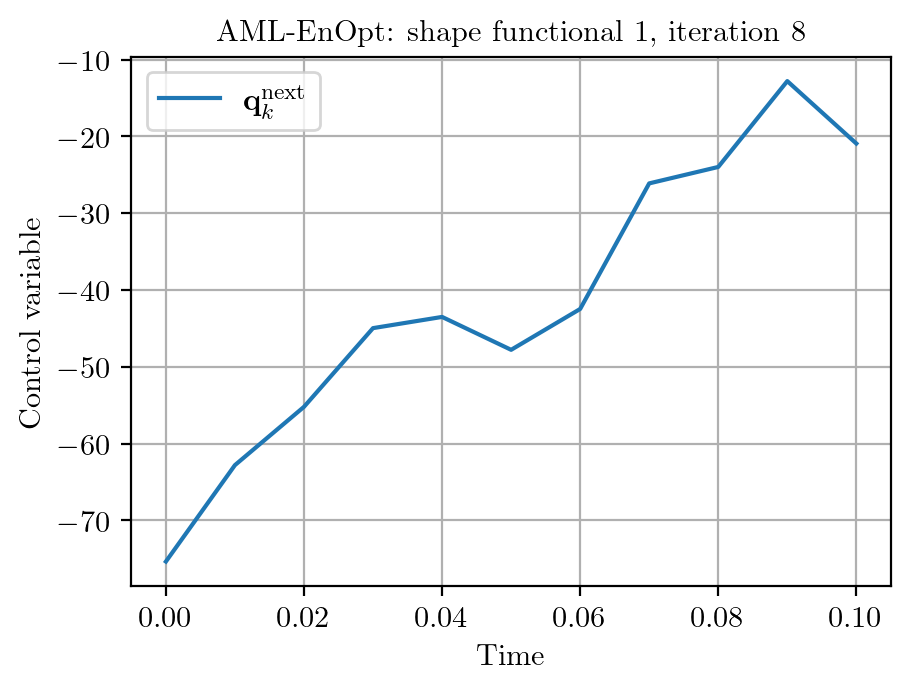
\includegraphics{Plots/noTRIteration8.png}
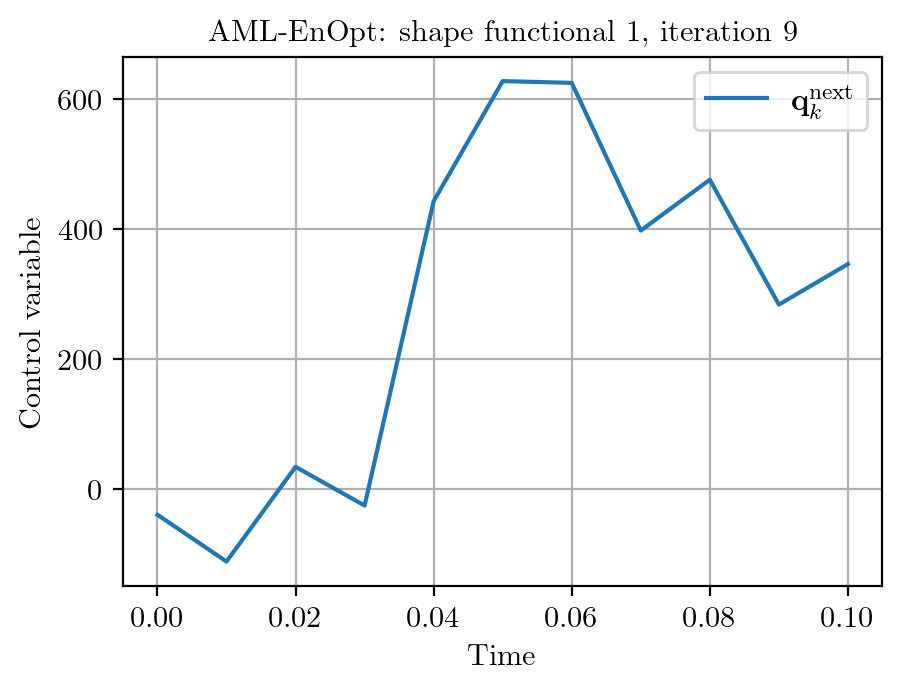
\includegraphics{Plots/noTRIteration9.png}
\caption{\label{noTRResults}An example of iterates after the eighth and ninth outer iteration if the trust region method is not applied}
\end{figure}